% Source: 2006浙江文.pdf, source-relative PDF page 1, Q17.
% Vertex labels and solid/dashed edge relationships follow the printed projection.
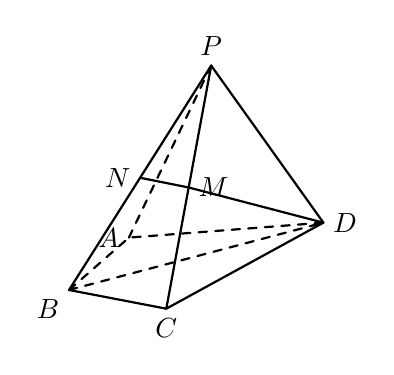
\begin{tikzpicture}[line cap=round,line join=round,x=0.95cm,y=0.95cm]
  \coordinate (P) at (1.65,3.15);
  \coordinate (A) at (0.55,0.85);
  \coordinate (B) at (-0.25,0.15);
  \coordinate (C) at (1.05,-0.1);
  \coordinate (D) at (3.15,1.05);
  \coordinate (N) at (0.7,1.65);
  \coordinate (M) at (1.35,1.52);
  \draw[thick] (P)--(B)--(C)--(D)--cycle;
  \draw[thick] (P)--(C) (N)--(M)--(D);
  \draw[thick,dashed] (P)--(A) (B)--(A)--(D) (B)--(D);
  \node[above] at (P) {$P$};
  \node[left] at (A) {$A$};
  \node[below left] at (B) {$B$};
  \node[below] at (C) {$C$};
  \node[right] at (D) {$D$};
  \node[left] at (N) {$N$};
  \node[right] at (M) {$M$};
\end{tikzpicture}
